\chapter{Introduction}

\textbf{What is a fusion plasma and why is it magnetically confined for nuclear fusion devices?}

A fusion plasma is a fully ionized gas whose behavior is dominated by long-range electric and magnetic fields. A major consequence of this behavior is that a plasma is an exceptionally good conductor of electricity, its conductivity implies that the plasma inside is shielded from DC electric fields $\bar{E}$ to a very large degree. On the other hand, DC magnetic fields $\bar{B}$ can penetrate and it is these fields that provide plasma confinement, hence the name "magnetic confinement" ~\cite[Chapter~6]{Freidberg2007}.\smallskip

\textbf{Why do we need magnetic fields in nuclear fusion devices ?}
\smallskip

Magnetic fields are needed to confine the hot plasma and keep it away from the machine walls.  In a generic magnetic fusion reactor the basic properties of magnetic fields require  a toroidal geometry so it can hold the plasma equilibrium ~\cite[Chapter~4]{Freidberg2007}. The properties of the magnetic fields require a toroidal geometry for confining magnetically the plasma. Trajectories of particles in the presence of magnetic fields are described by the Lorentz force equation $m \frac{d\bar{v}}{dt}=q(\bar{E}+\bar{v}\times \bar{B})$, which implies $\frac{d\bar{r}}{dt}=\bar{v}$, the combined perpendicular and parallel motion of a charged particle corresponds to a helical trajectory as  depicted in figure ~\ref{Helical}. If particles stream in a cylindrical device, they would collide with the wall due to the motion of the particles, a magnetic device whose lines wrapped around  a toroidal shape  prevent free streaming end loss, making obvious why the magnetic geometry for confining the plasma has to be toroidal.\smallskip

\begin{figure}
	\centering
	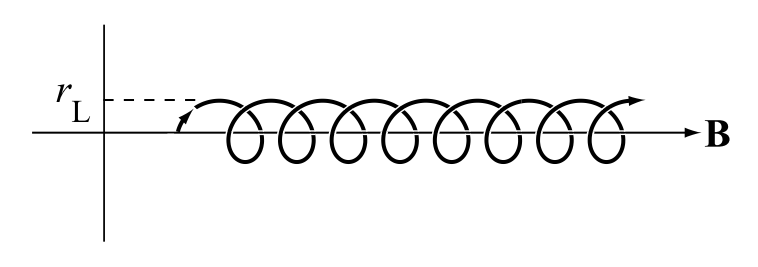
\includegraphics[width=0.525\textwidth]{Chp1/Helical_tray.png}
	\caption{  Helical trajectory of a charged particle in a uniform magnetic field ~\cite[Chapter~8]{Freidberg2007}.\label{Helical}}
\end{figure}

\section{Behind the plasma current}

Considering the drift of guiding center of a charged partice in a simple toroidal field in cylindrical coordinates $(R,\varphi,z)$. The component of the magnetic field $B_\varphi$ is the toroidal field and it decreases in the for of 1/R outward. The magnetic lines of force are circles around z axis. Particles in this  torus run fast in the toroidal direction and drift slowly in the z direction as shown in figure~\ref{TDrift}, this drift is called toroidal drift. As a consequence  using only a toroidal component of magnetic field is not sufficient for confining the plasma inside a toroidal device or a tokamak  since particles drift and therefore cause a loss of confinement ~\cite[Chapter~3]{Miyamoto2011}.\smallskip


\begin{figure}
	\centering
	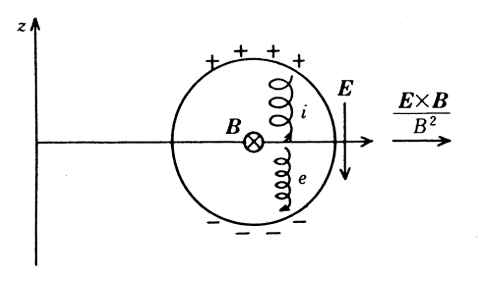
\includegraphics[width=0.55\textwidth]{Chp1/ToroidalDrift.png}
	\caption{Toroidal drift, particles drift in the vertical direction. ~\cite[Chapter~3]{Miyamoto2011} \label{TDrift}}
\end{figure}



If a current is induced in a toroidal plasma, the component of magnetic field around the magnetic axis (which is also called minor axis) is introduced. This component $B_P$ is called poloidal magnetic field and has components in $(R,z)$. The addition of this field creates magnetic lines circling the major axis of the torus, thus the particles circulate through the force lines. These lines cross a certain cross-section $P$ of the torus, each time the lines cross the plane $P$, the crossing point rotates around the minor axis by a certain angle $\iota$ which is called "rotational transform angle", this is shown in figure ~\ref{rot_angle}. The combination of toroidal and poloidal magnetic fields avoids the drift  described before originated by having an only-toroidal magnetic field by introducing a rotational transform angle. The poloidal field in a tokamak is mainly produced by the induced plasma toroidal current.  \smallskip

\begin{figure}
	\centering
	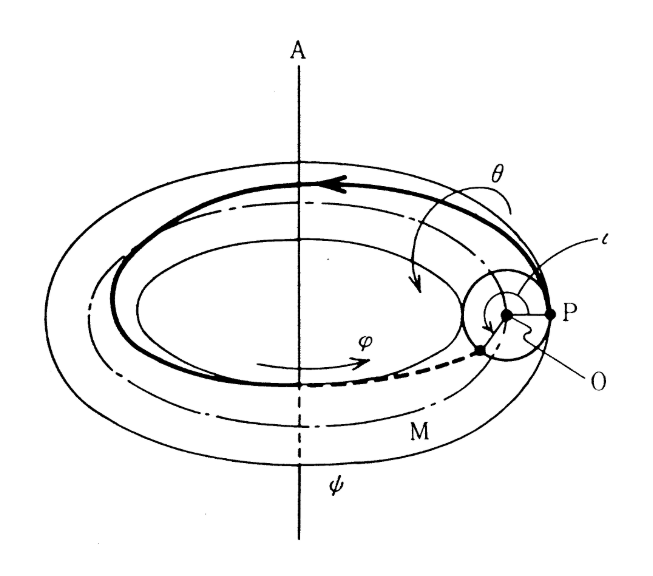
\includegraphics[width=0.655\textwidth]{Chp1/rotational_angle.png}
	\caption{Rotational transform angle $\iota$ formed when the magnetic force lines generated by the combination of toroidal and poloidal field cross the plane $P$ in different points  ~\cite[Chapter~3]{Miyamoto2011}. \label{rot_angle}}
\end{figure}

 All toroidal plasmas experience  outward toroidal forces along the $R$ direction, the first one is called the "hoop force" and is analogous to  the outward expansion force generated by the current flowing in a circular loop of wire, for this case corresponds to the toroidal current flowing in the plasma or simply called plasma current $I_p$. The second force is called "1/R force" and its name comes from the 1/R dependence of the toroidal field resulting from the toroidal geometry, the applied toroidal field $B_{\phi a}$,  where $a$ is the minor radius of the tokamak or the distance from the center of the vacuum chamber to the wall, has a 1/R dependence which follows from integrating Ampere's law around any closed toroidal loop located between the toroidal coils and the plasma. Finally the third one is called "tire tube force" and its existence is related to the difference of plasma pressures created by the toroidal geometry ~\cite[Chapter~11]{Freidberg2007}. \smallskip 
 
Given this outward toroidal forces, somehow the  toroidal force balance must be establish before the plasma hits the walls. An inwardly pointing restoring force is required and it is apply by means of the external poloidal field (PF) coils which generate a vertical field in order to compensate the radial forces generated by the tokamak. 
By choosing the magnitude and sign of the vertical field correctly, one can produce an inward restoring force to produce toroidal force balance. In order to make an analytic deviation of the toroidal force balance a simple model for the magnetic fields is used, this model consists of a toroidal plasma whose contours of constant pressure are a set of nested concentric circles $p=p(r)$ , where $r$ is the minor radius coordinate as shown in figure~\ref{tor_geo}. The simplified version of the pressure and magnetic fields to be used in the determination of the toridal force balance are:

	\begin{equation}
	\begin{aligned}
	p=&p(r)\\
	B =& \frac{R_0}{R}B_{\phi}(r) \hat{\phi} + \frac{R_0}{R}B_{\theta}(r)\hat{\theta}+B_v \hat{z}
	\end{aligned}
	\end{equation}
	
where $R_0$ is the tokamak major radius or the distance from the center of the torus to the center of the chamber (see figure ~\ref{tor_geo}), $B_{\theta}$ is the poloidal field and $B_v$ the external vertical field. After substituting the expression for the magnetic field into the general MHD force balance equation or Grad-Shafranov equation (~\cite[Chapter~6]{Miyamoto2011},~\cite[Chapter~11]{Freidberg2007},~\cite[Chpater~2]{Zohm2015}), the expression for the toroidal force balance can be obtained.
\smallskip

\begin{figure}
	\centering
	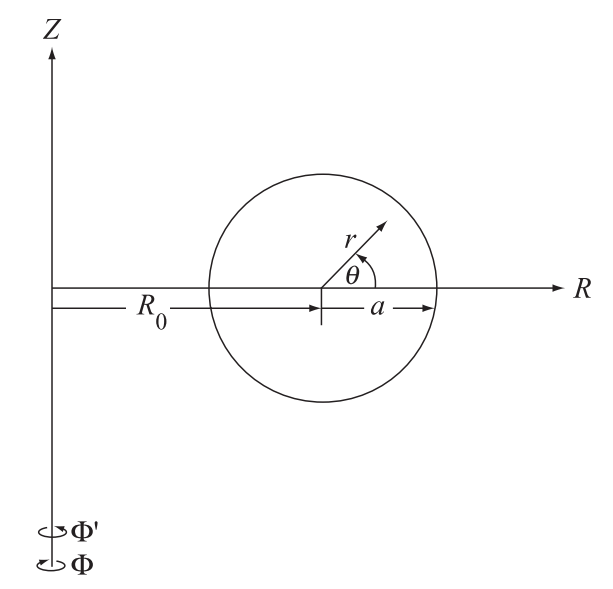
\includegraphics[width=0.6\textwidth]{Chp1/toroidal_geo.png}
	\caption{  Toroidal geometry and variables used for the calculations of the toroidal force balance and the vertical field~\cite[Chapter~11]{Freidberg2007}.\label{tor_geo}}
\end{figure}
%this is achieved by means of the application of an external vertical field.$


The toroidal force balance established the forces equation $F_{hoop}+ F_{1/R} + F_{tube}+ F_{v} =0$, where $F_v$ is the force generated by the external vertical field. Thus, the hoop force is given by:

\begin{equation}
F_{hoop}=2\pi^2a^2(li+le+2)~\frac{B_{\theta a}^2}{2\mu_0}
\end{equation}
 where $le$ and $li$ are the external and internal normalized inductances, $l= (L/2\pi R_0)/(\mu_0/4\pi)$. The "1/R" force is established as:
 
 \begin{equation}
 F_{1/R}=2\pi^2a^2 \left(\frac{ B_{\phi a}^2}{2\mu_0 }-\frac{\langle B_{\phi}^2 \rangle}{ 2\mu_0}\right)
 \end{equation}

where $\langle B_{\phi}^2 \rangle$ is the toroidal field average. The "tire tube" force is given by:
\begin{equation}
F_{tube}=2\pi^2a^2\langle p \rangle
\end{equation}

and finally the external vertical force is:

\begin{equation}
F_v=-2\pi^2a^2\left(\frac{2R_0 B_v B_{\theta a}}{a\mu_0}\right)
\end{equation}
 where $B_v$ is the external vertical magnetic field. Doing the combination of the 4 forces into the forces equation, the required vertical field for toroidal force balance remains:
 
 \begin{equation}
 B_v=B_{\theta a} ~\frac{a}{4R_0}\left[ \frac{2\mu_0 \langle p \rangle }{ B_{\theta a}^2} ~+~\frac{ B_{\phi a}^2 - \langle B_{\phi}^2 \rangle }{B_{\theta a}^2 } +li+le+2 \right]
 \label{force_balance}
 \end{equation}
  $B_v$ is the necessary vertical external field in order to avoid the plasma moving outwardly and touch the chamber walls, this equation will be addressed in chapter 4. In a purely vertical field, the plasma does not experience a vertical force and the vertical position is not well defined \cite[Chapter~4]{Zohm2015}\smallskip. Due to the form  PF coils are positioned around the vessel (see figure) the field produced by them is not completely vertical generating thus a radial component of the external magnetic field  due to Lorentz force law which  causes a vertical displacement of the plasma, this is compensated by adding another set of PF coils which generates an horizontal magnetic field.\smallskip
  
  
\section{Tokamak plasma control}

Tokamaks are basically devices with an axisymmetric configuration with a large toroidal magnetic field and a DC toroidal current, given its physical characteristics and its performance until now is presently the leading candidate to become the world’s first fusion reactor. During the start up and subsequent approximately steady state phase of many fusion plasma discharges a toroidal current is induced in the plasma by means of transformer action with the plasma being the secondary of the transformer  ~\cite[Chapter~9]{Freidberg2007}. Sometimes “poloidal field coils” means both the equilibrium field coils and the ohmic heating coils. By raising the current of the primary windings of the current transformer (ohmic heating coils), a current is induced in the plasma, which acts as the secondary winding. \smallskip

Typical operation of a tokamak discharge starts with the establishment of a large, steady, toroidal, magnetic field. Next, neutral gas is injected into the vacuum chamber and often pre-ionized. The transformer induced toroidal current or simply called plasma current $I_p$ is then ramped up to its maximum value and maintained for the “flat top” portion of the pulse~\cite[Chapter~13]{Freidberg2007}.\smallskip

Control engineering for magnetic confined plasmas  embrace different types of techniques and they are use for  controlling different kind of variables and characteristics of the device and the plasma. One of the main tasks of control engineering in the field of fusion is to maintain the plasma in certain position and shape in such way that it stays stable, follows set-points and rejects possible instabilities which may occur maintaining a constant plasma current.\smallskip  


\section{Thesis outline}

This thesis will study the properties and control applications for two tokamaks: JT60-SA and ISTTOK. These tokamaks possess physical characteristics which vary in big scale between them: the size, ISTTOK has cross-circular section and JT60-SA is a diverted plasma, the dimension of the magnetic fields, ISTTOK has 30 years operating and JT60-SA will start operations in 2020, etc. Despite this facts there exist a reason to join the two machines in a single work, both tokamaks rely on active magnetic control applied to the PF coils in order to control the plasma position and shape.  This work is divided in 5 chapters.\smallskip

$\bullet$ Chapter 2 explores the plasma control systems implemented in different tokamaks around the world and addresses some important theoretical concepts to be applied in the further chapters.\smallskip

$\bullet$ Chapter 3 JT60-SA \smallskip

$\bullet$ Chapter 4 ISTTOK tokamak \smallskip

$\bullet$ Chapter 5 Control results in ISTTOK. \smallskip


The main objectives of this thesis is to achieve an implementation 